\cleardoublepage
\chapter{Introduction}
\label{sec:intro}
\pagenumbering{arabic} % para empezar la numeración de página con números

\section{General context}

An Unmanned Aerial Vehicle (UAV) is an aircraft able to fly without any pilot or operator on board. They may be operated through remote control by a human operator or with various degrees of autonomy, from sensor-driven control aids provided to the operator to fully autonomous flight through preplanned missions.
UAVs have existed since the 20th century and were initially developed as military technology to protect pilots from dangerous missions.
However, as the cost of the electronics and sensors decreased and control technologies were improved, they became available to a broader public and are now employed in a wide range of civil applications like crop control, search and rescue, or filmmaking and photography.
Nevertheless, most commercial solutions are limited to remote operations or basic autonomy, with fully autonomous flight still in the earliest phases.
However, there is a growing trend towards using vision-based control solutions, which can offer improved performance and flexibility compared to traditional control methods.
Vision-based control solutions use cameras and image processing algorithms to provide real-time feedback and control of the UAV. 
These solutions are often more flexible and robust than traditional control methods, which are typically based on accelerometers, gyroscopes, and other sensors. 
Additionally, vision-based control solutions can be implemented on low-cost platforms, making them accessible to a wider range of users.
These vision-based guidance systems have only started to appear in recent years as artificial intelligence becomes more widespread and very few fully-developed consumer-ready platforms are available for the general public.
Even so,
from the essential hardware to build your own quadcopter, a helicopter with four rotors that represents the most common type of UAV, to miniaturized computers that handle complex calculations and open-source software that can be customized to endless applications,
all the individual pieces that enable building such a system are readily available.

\section{The Dronecontrol project}

The project presented in this thesis aims to show the options available to design and implement control solutions for the popular PX4 open-source autopilot platform and how to integrate them with detection and tracking computer vision mechanisms to achieve simple vision-based self-guided UAVs.
All the necessary code for this project has been written in the Python programming language and always runs outside of the flight controller board on a companion computer.
This allows more processing power to be accessible for any compute-intensive computer vision algorithms,
but also ensures that the control solutions are abstracted from the hardware components and not dependent on the specific flight stack employed, 
to allow applying the results to any available autopilot platform with exposed APIs.
Two complete vision-based control solutions have been implemented for two different scenarios: keeping the computer driving the computer vision algorithms on board or off-board the vehicle itself during flight.
The following chapters detail the hardware, libraries, testing environments, and systems used during the development process and how they can be used to develop new control solutions based on available computer vision mechanisms.


%%-- Objetivos del  proyecto
%%-- Si la sección anterior ha quedado muy extensa, se puede considerar convertir
%%-- Las siguientes tres secciones en un capítulo independiente de la memoria

\section{Objectives}
\label{sec:objetives}

The main objective of this project is to demonstrate the available possibilities to develop control solutions for the PX4 autopilot driven by computer vision mechanisms.

More specifically, it aims to:
\begin{itemize}
    \item Introduce the software and hardware environment of the Dronecode project and the techniques they have made available.
    \item Show the minimum requirements needed to develop control software for the platform.
    \item Suggest viable vision-driven control solutions that use those techniques.
    \item Present a testing process using available tools that can help ensure safety and reliability for any new solutions developed.
    \item Build a quadcopter and use it to carry out test flights with the developed solutions.
\end{itemize}


\section{Time planning}
\label{sec:time-planning}
\todo[inline]{Write: time planning}

% Es conveniente que incluyas una descripción de lo que te ha llevado realizar el trabajo.
% Hay gente que añade un diagrama de GANTT.
% Lo importante es que quede claro cuánto tiempo has consumido en realizar el TFG/TFM 
% (tiempo natural, p.ej., 6 meses) y a qué nivel de esfuerzo (p.ej., principalmente los 
% fines de semana).

\begin{figure}
  \centering
  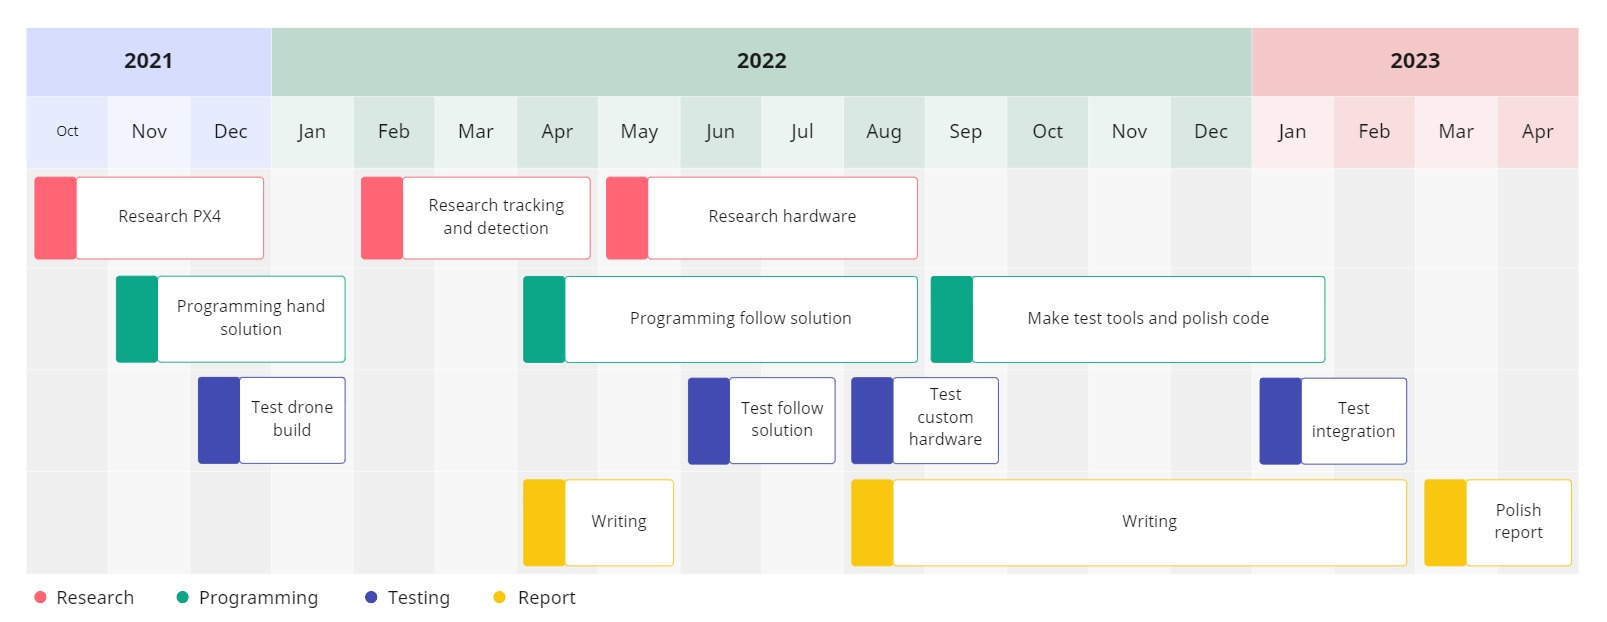
\includegraphics[width=\textwidth,keepaspectratio]{img/project-timeline.jpg}
  \caption{High-level overview of how different components interact in the AirSim simulator.}
  \label{fig:project-timeline}
\end{figure}


- Phase 1: Research on PX4, openCV, existing vision-based control solutions and research (Oct-Dec 21) 10 hours
- Phase 2: Development of hand solution (Nov 21 - Jan 22) 51 hours
- Phase 3: Research object tracking and Airsim (Feb 22 - Apr 22)
- Phase 4: Development of follow solution (Apr 22 - Aug 22)
- Phase 5: Research Raspberry Pi and hardware (May 22 - Aug 22)
- Phase 6: Testing (Dec21, June 22 - Sep 22)
--- Writing: (Apr-May 22, Aug 22 - Mar 23)

\section{Thesis layout}
\label{sec:layout}

This section details the structure of this thesis.
The work is composed of five individual chapters that reflect the four distinct phases described in the last section.

\begin{itemize}
    \item In the first chapter, there is a brief introduction to the context in which the project has been developed, as well as the objectives it pursues.
    \item Chapter 2 presents the technologies and tools employed in this project and the current state-of-the-art of vision-based control solutions for UAVs.
    \item The third chapter introduces the simulation environments used to develop the solutions throughout the entire project and the architecture of both the hardware used and the software developed.
    \item Chapter 4 follows along through the process of testing every part of the system incrementally until reaching the final flight tests.
    \item The last chapter shows the conclusions drawn from the work and presents ideas for future development.
\end{itemize}


\cleardoublepage